\documentclass[12pt]{article}
\usepackage{setspace}
\usepackage{a4}
\usepackage{amssymb,amsmath,amsthm,latexsym}
\usepackage{amsfonts}
\usepackage{amsfonts}
\usepackage{array}
\usepackage[numbers]{natbib}
\bibliographystyle{plainnat}
\usepackage{float}
\usepackage[nottoc]{tocbibind}
\setlength{\parindent}{1.0cm} \setlength{\evensidemargin}{0.0cm}
\setlength{\oddsidemargin}{0.0cm} \setlength{\topmargin}{0.0cm}

\textwidth 17cm \textheight 20cm
\onehalfspacing



\usepackage{microtype}
\usepackage{tablefootnote}
\usepackage{threeparttable}  
\usepackage{booktabs}
\usepackage{caption}
\captionsetup{justification   = raggedright,
              singlelinecheck = false}
\usepackage{bm}
\usepackage{stfloats}
\usepackage{mathrsfs}
\usepackage{tabularx}
%\usepackage{algpseudocode}
\usepackage{array}
\usepackage{multirow}
\usepackage{nicematrix}
\usepackage[thinlines]{easytable}
\usepackage{enumitem}
\usepackage{textcomp}
\usepackage{subcaption}

\usepackage{amsmath}
\usepackage{adjustbox}
\usepackage{graphicx}
\usepackage{float}
\usepackage{graphicx}
\captionsetup[subfigure]{font=footnotesize}
\makeatletter
\usepackage{listings}
\usepackage{color}

\definecolor{dkgreen}{rgb}{0,0.6,0}
\definecolor{gray}{rgb}{0.5,0.5,0.5}
\definecolor{mauve}{rgb}{0.58,0,0.82}
\lstset{frame=tb,
  language=Java,
  aboveskip=3mm,
  belowskip=3mm,
  showstringspaces=false,
  columns=flexible,
  basicstyle={\small\ttfamily},
  numbers=none,
  numberstyle=\tiny\color{gray},
  keywordstyle=\color{blue},
  commentstyle=\color{dkgreen},
  stringstyle=\color{mauve},
  breaklines=true,
  breakatwhitespace=true,
}

\usepackage[justification=centering]{caption}

\usepackage{multicol}
\usepackage{longtable}
%\usepackage{biblatex}

\usepackage{algorithm,algorithmic}
\def\newblock{\hskip .11em plus .33em minus .07em}
\def\BibTeX{{\rm B\kern-.05em{\sc i\kern-.025em b}\kern-.08em
		T\kern-.1667em\lower.7ex\hbox{E}\kern-.125emX}}





\usepackage[justification=centering]{caption}

\usepackage{multicol}
\usepackage{longtable}

\AtBeginEnvironment{procedure}{\let\c@algocf\c@procedure}
\makeatother

%\usepackage{natbib}
\usepackage{tablefootnote}
\usepackage{threeparttable}  
\usepackage{multirow}
\usepackage{textcomp}
\newtheorem{definition}{Definition}
\usepackage{subcaption}
\usepackage{adjustbox}
\usepackage{graphicx}
\usepackage{graphics}
\usepackage{float}
\usepackage{etoolbox}
\newcounter{procedure}
\makeatletter
\AtBeginEnvironment{procedure}{\let\c@algocf\c@procedure}
\makeatother
\usepackage[font=footnotesize]{caption}
\captionsetup[table]{labelsep=newline}
%\captionsetup[ruled]{labelsep=period}
\captionsetup[figure]{labelsep=period}
%\captionsetup[subfigure]{labelsep=period}
\captionsetup[subfigure]{font=footnotesize}
\makeatletter
\usepackage{algorithm,algorithmic}
\def\newblock{\hskip .11em plus .33em minus .07em}
\def\BibTeX{{\rm B\kern-.05em{\sc i\kern-.025em b}\kern-.08em
		T\kern-.1667em\lower.7ex\hbox{E}\kern-.125emX}}
%\usepackage{algorithmicx}
\usepackage{amssymb}
\usepackage{float}
\usepackage{amsthm,xpatch,amsmath}
\usepackage{amsmath}
\makeatletter
\xpatchcmd{\@thm}{\fontseries\mddefault\upshape}{}{}{} % same font as thm-header
\makeatother
%\theoremstyle{definition}
%\newtheorem{definition}{Definition}
%\theoremstyle{example}
%\newtheorem{example}{Example}
%\theoremstyle{lemma}
\newtheorem{lemma}{Lemma}
\usepackage{listings}
\usepackage{color}
\definecolor{dkgreen}{rgb}{0,0.6,0}
\definecolor{gray}{rgb}{0.5,0.5,0.5}
\definecolor{mauve}{rgb}{0.58,0,0.82}
\lstset{frame=tb,
  language=Java,
  aboveskip=3mm,
  belowskip=3mm,
  showstringspaces=false,
  columns=flexible,
  basicstyle={\small\ttfamily},
  numbers=none,
  numberstyle=\tiny\color{gray},
  keywordstyle=\color{blue},
  commentstyle=\color{dkgreen},
  stringstyle=\color{mauve},
  breaklines=true,
  breakatwhitespace=true,} 
\newcommand*{\comb}[2]{{}^{#1}C_{#2}}%
\newcommand{\RNum}[1]{\lowercase\expandafter{\romannumeral #1\relax}}
\makeatletter
\@dblfptop 0pt
\makeatother







\usepackage{url}
\newcommand{\tmx}{\ensuremath{\times}}
\renewcommand{\topfraction}{0.9}
\renewcommand{\bottomfraction}{0.8}
\renewcommand{\textfraction}{0.1}
\renewcommand{\floatpagefraction}{0.75}
\setcounter{topnumber}{3}
\setcounter{bottomnumber}{2}
\setcounter{totalnumber}{5}

\begin{document}
\begin{titlepage}
\doublespacing

\begin{center}
\par {\large \textbf{Mini Project Report}}\\
\end{center}

\begin{center}
	\par {\large \textbf{on}}
\end{center}

\begin{center}
{\Large \textbf{Memory Architectures of AI Inference Chips: Cycle-Accurate Evaluation and Access-Pattern Analysis}}
\end{center}

{\small
\begin{center}
\par \small {Submitted by}
\par \Large \textbf{G. V. Prajwal} \textbf{(23bcs048)}
\par \Large \textbf{Siddhaartha B. S.} \textbf{(23bcs127)}
\par \Large \textbf{Yogeshgouda Patil} \textbf{(23bcs138)}
\par \normalsize Under the guidance of
\par \large \textbf{Dr. Prabhu Prasad B M}
\par \textbf{Assistant Professor}
\end{center}
}

\begin{figure}[h]
\begin{center}
\IfFileExists{iiIT-Dharwad-Logo-horizontal-500x154[1].png}{%

\includegraphics[height=.80in]{iiIT-Dharwad-Logo-horizontal-500x154[1].png}}{%
\fbox{\parbox[c][.6in][c]{3.2in}{\centering\scriptsize Place the IIIT Dharwad logo file\\ \texttt{iiIT-Dharwad-Logo-horizontal-500x154[1].png}\\ in the project folder}}}
\end{center}
\end{figure}

\begin{center}
\par{\mbox {\small\textbf{DEPARTMENT OF COMPUTER SCIENCE AND ENGINEERING}}}
\noindent{\mbox{\small \textbf{ INDIAN INSTITUTE OF INFORMATION TECHNOLOGY
DHARWAD}}}\\
20/11/2026

\end{center}
\end{titlepage}


\newpage
\thispagestyle{empty}
\clearpage
\thispagestyle{empty}
\phantom{a}
\newpage
\thispagestyle{empty}

\begin{center}
	\emph{\huge{Certificate}}\\[2.5cm]
\end{center}
\normalsize This is to certify that the project, entitled \textbf{Memory Architectures of AI Inference Chips: Cycle-Accurate Evaluation and Access-Pattern Analysis}, is a bonafide record of the Mini Project coursework presented by the students whose names are given below during the academic year 2026--2027 in partial fulfilment of the requirements of the degree of Bachelor of Technology in Computer Science and Engineering.\\[1.0cm]

\begin{table}[h]
	\centering
	\begin{tabular}{lr}
		Roll No & Names of Students \\ \\ \hline
		\\
		23bcs048 & G. V. Prajwal \\
		23bcs127 & Siddhaartha B. S. \\
		23bcs138 & Yogeshgouda Patil \\
	\end{tabular}
\end{table}

\vfill

\begin{flushright}
	Dr. Prabhu Prasad B M\\
	(Project Supervisor)\\[1.5cm]
\end{flushright}

\newpage
\pagenumbering{roman}
\setcounter{page}{1}
\tableofcontents
\newpage
\listoffigures
\newpage
\listoftables


\newpage
\thispagestyle{empty}
\clearpage
\thispagestyle{empty}
\phantom{a}
\newpage

%=====================================================================
\section{Introduction}
\pagenumbering{arabic}
%=====================================================================
Large-language-model (LLM) inference is limited by data movement more than by arithmetic~\cite{wulf1995,gholami2024}. When a model generates one token at batch size~1, it reads all of its weights and its key--value (KV) cache once, so the time per token is set by how fast memory can deliver bytes. Chip designers have answered this with very different memory systems:
\begin{itemize}
\item GPUs pair a modest on-chip cache with high-bandwidth memory (HBM)~\cite{choquette2023};
\item dataflow meshes and NPUs pair a large, compiler-managed SRAM scratchpad with commodity GDDR6 or LPDDR5~\cite{vasiljevic2021};
\item SRAM-only designs, such as the Groq LPU~\cite{abts2020} and the Cerebras wafer-scale engine~\cite{lie2023}, remove DRAM and keep all state on chip.
\end{itemize}

Datasheet (``pin'') bandwidth hides three effects that decide real performance. First, the bandwidth a DRAM system actually \emph{achieves} depends on the access pattern: row-buffer locality, bank parallelism and refresh can lose most of the pin bandwidth on gathers. Second, the same memory systems are increasingly expected to run general-purpose code, whose irregular, latency-bound accesses differ sharply from inference streams. Third, \emph{how} requests arrive at the memory controllers determines how predictable memory access is: Agarwal \emph{et al.}~\cite{agarwal2025} showed that the power spectral density (PSD) of inter-arrival times at the memory controller characterises this predictability.

\subsection{Objectives}
The objective of this project is to explore the memory architecture of AI-inference chips and to compare them on different workloads. Specifically, we aim to:
\begin{enumerate}
\item describe seven memory-system archetypes with public-specification class parameters, and simulate their DRAM cycle-accurately;
\item measure how much of each DRAM technology's pin bandwidth survives realistic inference access patterns;
\item evaluate latency, chip count, throughput per chip and energy of twelve AI inference scenarios on each archetype;
\item evaluate how the same memory systems serve general-purpose code (SPEC CPU~2026), with the processor core held fixed;
\item characterise the memory access patterns of these programs and the predictability of the resulting request streams at the DRAM controllers.
\end{enumerate}

\subsection{Contributions}
The project contributes a reproducible framework (\texttt{memarch}) built on Ramulator~2.1, the current release of Ramulator~2.0~\cite{luo2024}; a per-access-pattern DRAM calibration feeding an operator-level inference model; an LLVM pass that turns C/C++ programs into L2-miss traces replayed on every memory system with an identical core; and a PSD-based classification of the DRAM request stream that extends~\cite{agarwal2025} with explicit thresholds and an anti-persistent class.

\subsection{Organisation of the Report}
Section~\ref{sec:related} reviews related work. Section~\ref{sec:methods} describes the data and methods: the architectures, workloads, simulator, models, tracer and analyses. Section~\ref{sec:results} presents and discusses the results, and Section~\ref{sec:conclusion} concludes.
\newpage

%=====================================================================
\section{Related Work}\label{sec:related}
%=====================================================================
\textbf{Memory-bound inference.} The memory wall~\cite{wulf1995} has become the main limit of transformer inference~\cite{gholami2024}. Paged KV caches~\cite{kwon2023} turn KV reads into page gathers, which is one of the access patterns studied here. The roofline model~\cite{williams2009} bounds performance by peak compute and peak bandwidth, and Pope \emph{et al.}~\cite{pope2023} model the partitioning of LLM inference across accelerators.

\textbf{Hardware evaluation frameworks.} LLMCompass~\cite{zhang2024} and GenZ~\cite{bambhaniya2024} model LLM inference hardware in more detail than this project (operator mapping, hybrid parallelism, on-chip tiling and interconnect topology), but use peak memory bandwidth. Our operator model is a simpler per-operator roofline that instead uses DRAM bandwidth measured per access pattern. We do not compare against these frameworks quantitatively.

\textbf{AI accelerator memory systems.} Accelerators range from the TPU's large on-chip buffer backed by DRAM~\cite{jouppi2017} to SRAM-only designs~\cite{abts2020,lie2023}; Tenstorrent's mesh~\cite{vasiljevic2021} pairs per-core SRAM with GDDR6, and NVIDIA's H100~\cite{choquette2023} uses HBM3. These designs are usually compared on vendor benchmarks; we compare their \emph{memory systems} under one model.

\textbf{Simulation and characterization.} Ramulator~\cite{kim2016,luo2024} provides cycle-accurate models of DRAM standards and controllers, including FR-FCFS scheduling~\cite{rixner2000}; we use it both to calibrate access patterns and as the memory back end of trace replay. SPEC suites have been characterised with binary instrumentation~\cite{luk2005} and hardware counters~\cite{limaye2018}; our tracer instead works at the LLVM IR level~\cite{lattner2004}, inside SPEC's own build harness.

\textbf{Predictability of memory traffic.} Bogdan \emph{et al.}~\cite{bogdan2010} showed that network-on-chip (NoC) traffic is non-stationary and fractal. Agarwal \emph{et al.}~\cite{agarwal2025} used the PSD of inter-packet arrival times at the memory controller to show how cache, buffer and network size change the predictability of memory access in NoC systems. We apply this analysis at the DRAM command level, across five DRAM technologies.
\newpage

%=====================================================================
\section{Data and Methods}\label{sec:methods}
%=====================================================================
Figure~\ref{fig:framework} summarises the framework. The AI study runs the same operator graphs on every chip class, using DRAM bandwidth measured in Ramulator. The SPEC study replays the same traces on the same core in front of every memory system. A third analysis records every DRAM command of those replays to characterise the request streams.

\begin{figure}[htbp]
\centering
\resizebox{\textwidth}{!}{\begin{tabular}{|c|c|c|}
\hline
\textbf{LLVM tracing} & \textbf{Ramulator 2.1} & \textbf{Analysis (Python)}\\
\hline
SPEC CPU 2026 sources & Bandwidth of 5 & Inference model:\\
$\downarrow$ clang -O2 + LLVM pass & access patterns $\rightarrow B_d(p)$ & chips, step time, energy\\
\hline
Tracer runtime: & Trace replay: & IPC, DRAM traffic,\\
skip, warm up, trace 200M & core + SRAM LLC + DRAM & latency, row hits\\
\hline
L2-miss trace & DRAM command recording & Locality; inter-request time,\\
$\langle$gap, address, dirty victim$\rangle$ & (every channel) & PSD slope $\beta$, class\\
\hline
\end{tabular}}
\caption{Framework overview. Each row flows left to right; the SPEC traces from the first column drive the trace replay in the second.}
\label{fig:framework}
\end{figure}

%---------------------------------------------------------------------
\subsection{Memory-System Archetypes}
Each archetype is one configuration file (Table~\ref{tab:arch}). Its values are public-specification \emph{class} values (orders of magnitude of shipping parts), not calibrated vendor models. The key distinction is the role of the on-chip SRAM:
\begin{itemize}
\item \textbf{cache} (CPU, GPU): hardware-managed least-recently-used (LRU) cache. A cyclic weight or KV stream larger than the cache misses on every access;
\item \textbf{scratchpad} (mesh, NPU): compiler-managed. Activations are pinned first, then as much persistent state as fits, and the rest streams from DRAM;
\item \textbf{resident} (LPU, wafer): there is no DRAM. All state lives in SRAM, so the number of chips is set by capacity.
\end{itemize}


\begin{table}[htbp]
\centering
\caption{Memory-system archetypes (public-specification class values; TFLOPS = bf16 peak). HBM3 pairs the bandwidth of 64 64-bit channels (4 stacks) with an 80\,GiB capacity.}
\label{tab:arch}
\scriptsize
\setlength{\tabcolsep}{3pt}
\resizebox{\textwidth}{!}{\begin{tabular}{@{}llllrrr@{}}
\toprule
Archetype & SRAM (role) & SRAM BW, latency & DRAM (ch.\,\tmx\,width, capacity, pin BW) & TFLOPS & Link GB/s & TDP W\\
\midrule
CPU + DDR5 & 96 MiB (cache) & 3 TB/s, 14 ns & DDR5-4800, 16\tmx32b, 512 GiB, 307 GB/s & 120 & 64 & 350\\
GPU + HBM3 & 50 MiB (cache) & 7 TB/s, 120 ns & HBM3 6.4\,Gb/s, 64\tmx64b, 80 GiB, 3,277 GB/s & 989 & 450 & 700\\
GPU + HBM4 & 128 MiB (cache) & 16 TB/s, 120 ns & HBM4 8\,Gb/s, 128\tmx64b, 288 GiB, 8,192 GB/s & 2,500 & 900 & 1,200\\
Mesh + SRAM + GDDR6 & 210 MiB (scratchpad) & 24 TB/s, 60 ns & GDDR6 14\,Gb/s, 8\tmx32b, 32 GiB, 448 GB/s & 370 & 400 & 300\\
NPU + SRAM + LPDDR5 & 144 MiB (scratchpad) & 12 TB/s, 40 ns & LPDDR5-6400, 8\tmx32b, 64 GiB, 205 GB/s & 200 & 32 & 75\\
LPU (SRAM only) & 230 MiB (resident) & 80 TB/s, 30 ns & none & 188 & 330 & 300\\
Wafer-scale SRAM & 44 GiB (resident) & 21,000 TB/s, 200 ns & none & 62,500 & 150 & 23,000\\
\bottomrule
\end{tabular}}
\end{table}



%---------------------------------------------------------------------
\subsection{Workloads}
\textbf{AI inference.} Twelve scenarios (Table~\ref{tab:scen}) cover dense LLMs, a mixture-of-experts (MoE) LLM, a CNN and a recommender. All use 16-bit weights. Unit tests check the parameter counts against the published models (8.03B, 70.6B, 46.7B and 25.5M parameters).

\begin{table}[htbp]
\centering
\caption{AI inference scenarios.}
\label{tab:scen}
\small
\resizebox{\textwidth}{!}{\begin{tabular}{@{}llrrl@{}}
\toprule
Scenario & Model & Batch & Context & Notes\\
\midrule
llama8b\_decode\_b1 / b32 & Llama-3.1-8B~\cite{llama3} & 1 / 32 & 2,048 & one token per sequence\\
llama8b\_decode\_longctx & Llama-3.1-8B & 8 & 32,768 & KV cache of 34\,GB\\
llama8b\_prefill & Llama-3.1-8B & 1 & 2,048 & whole prompt\\
llama70b\_decode\_b1 / b32 & Llama-3.1-70B & 1 / 32 & 2,048 / 4,096 & \\
llama70b\_prefill & Llama-3.1-70B & 1 & 2,048 & \\
mixtral\_decode\_b1 / b32 & Mixtral-8x7B~\cite{jiang2024} & 1 / 32 & 2,048 & top-2 of 8 experts\\
resnet50\_b1 / b64 & ResNet-50~\cite{he2016} & 1 / 64 & -- & 224\tmx224 images\\
dlrm\_b2048 & DLRM-DCNv2-style~\cite{naumov2019} & 2,048 & -- & 26 tables, 250M rows (64\,GB)\\
\bottomrule
\end{tabular}}
\end{table}

\textbf{General-purpose code.} Eight C/C++ rate benchmarks of SPEC CPU~2026~\cite{spec2026} were selected for varied memory behaviour (Table~\ref{tab:traces}). The host has no Fortran compiler, so Fortran benchmarks were excluded. Each benchmark runs its first \texttt{refrate} workload; these are measurement runs, not reportable SPEC results.

\begin{table}[htbp]
\centering
\caption{SPEC CPU 2026 traces (200M traced instructions each).}
\label{tab:traces}
\small
\resizebox{\textwidth}{!}{\begin{tabular}{@{}llrrrr@{}}
\toprule
Benchmark & Domain & L2 MPKI & Dirty WB/miss & Window MiB & Peak RSS MiB\\
\midrule
706.stockfish\_r & chess search, hash tables & 0.39 & 77\% & 274 & 1,799\\
708.sqlite\_r & database & 2.34 & 57\% & 20 & 461\\
710.omnetpp\_r & discrete-event simulation & 5.47 & 27\% & 17 & 111\\
750.sealcrypto\_r & homomorphic encryption & 2.63 & 51\% & 15 & 538\\
767.nest\_r & spiking neural networks & 11.47 & 58\% & 69 & 1,169\\
772.marian\_r & neural machine translation & 0.15 & 29\% & 3 & 703\\
777.zstd\_r & compression & 1.19 & 19\% & 12 & 397\\
782.lbm\_r & lattice-Boltzmann fluids & 57.89 & 75\% & 542 & 1,767\\
\bottomrule
\end{tabular}}
\end{table}

%---------------------------------------------------------------------
\subsection{Cycle-Accurate DRAM Model (Ramulator 2.1)}
Each DRAM system is simulated in Ramulator~2.1 (built from source at commit \texttt{7bead6c}) through its C++ simulation loop, with one controller per channel: FR-FCFS scheduling~\cite{rixner2000}, open-row policy, refresh enabled and 64-entry read and write queues. Consecutive 64\,B lines are interleaved across channels, and within a channel the MOP4CLXOR mapping spreads them over banks and rows. Integrating the simulator required several fixes: a bank-group-aware address mapping (which lifts an HBM3 stream from 51\% to 99\% of pin bandwidth), ganging narrow LPDDR5/GDDR6 channels into 32-bit pairs, two back-to-back bursts for 64\,B requests on HBM pseudo-channels, missing GDDR6 refresh timings, power-of-two LLC set counts, and using HBM's half-rate controller clock in all timing conversions.



\textbf{Access-pattern calibration.} For each DRAM system, five synthetic traces (each at least 120k requests) are replayed with Ramulator's load--store frontend: sequential reads (weight streaming), 2:1 read/write streams (activations, KV appends), random 4\,KiB pages read sequentially (paged KV cache), random 256\,B rows (embedding lookups) and uniform random 64\,B lines. The sustained bandwidth $B_d(p)$ of DRAM system $d$ for pattern $p$, summed over channels, is stored for the inference model.

%---------------------------------------------------------------------
\subsection{Inference Performance Model}
The inference model is an operator-level roofline~\cite{williams2009} on top of the calibrated DRAM. Each traffic class uses the pattern it resembles: weights a sequential stream, KV reads 4\,KiB page gathers, KV writes and activations a 2:1 read/write stream, and embeddings 256\,B row gathers.

\textbf{Chip count.} A model with persistent state $P$ (weights, KV cache, embedding tables) and peak activations $A$ is spread over the fewest chips that hold it, with 90\% of the capacity $C$ per chip usable ($C$ is the DRAM capacity, or the SRAM capacity for SRAM-only designs):
\begin{equation}
n = \left\lceil \frac{P + A}{0.9\, C} \right\rceil .\label{eq:chips}
\end{equation}

\textbf{Placement.} A resident SRAM serves all bytes. A scratchpad holds all activations if they fit (otherwise all activation traffic goes to DRAM) and then as much persistent state as fits; the rest streams from DRAM. A cache serves persistent state only if all of it fits; GPU shared memory and hot-row caching of skewed embedding tables are not modelled. For the MoE model, $P$ counts all experts, while traffic counts only the expected number of distinct active experts, $8[1-(1-2/8)^{t}]$ for $t$ tokens.

\textbf{Step time.} One inference step executes the model's fused operators $o$ in order (four per transformer layer plus embedding and output layers: 130 for Llama-8B, 322 for Llama-70B, 162 for Mixtral, 54 for ResNet-50), each split across all $n$ chips (pure tensor parallelism):
\begin{equation}
T = \sum_{o} \Big[\max\big(t^{\mathrm{comp}}_o,\ t^{\mathrm{mem}}_o\big) + t^{\mathrm{comm}}_o + \tau\Big],\label{eq:step}
\end{equation}
with four terms per operator:
\begin{itemize}
\item $t^{\mathrm{comp}}_o = F_o/(n\,\Pi)$: the operator's FLOPs $F_o$, split over $n$ chips, at the chip's effective FLOP rate $\Pi$ (matrix peak times the efficiency in Table~\ref{tab:const}; half the vector peak for vector operators);
\item $t^{\mathrm{mem}}_o = \sum_p D_{o,p}/(n\,B_d(p))$: its DRAM bytes in each access pattern $p$, split over $n$ chips, at the bandwidth \emph{measured for that pattern}. SRAM bytes are timed the same way with the SRAM bandwidth; the SRAM and DRAM paths run in parallel and the slower one counts;
\item $t^{\mathrm{comm}}_o$: the collective after the operator when $n>1$. An all-reduce of $M$ bytes takes $2\lceil\log_2 n\rceil h + 2\frac{n-1}{n}\frac{M}{L}$ with hop latency $h$ and link bandwidth $L$~\cite{thakur2005}; each transformer layer needs two (65 for Llama-8B). DLRM's embeddings use one all-to-all, $\lceil\log_2 n\rceil h + \frac{n-1}{n^2}\frac{M}{L}$;
\item $\tau$: a fixed launch or synchronization overhead per operator.
\end{itemize}
Compute and memory overlap, so the slower of the two sets each operator's time. At batch~1, decode reads every weight once while doing little arithmetic, so $t^{\mathrm{mem}}$ dominates and $T$ is roughly the weight bytes divided by the measured stream bandwidth. A step is \emph{bound by} whichever of the four terms contributes most to $T$.

\textbf{Energy.} Dynamic energy per token counts the bits moved in SRAM, DRAM and links times their energy per bit (Table~\ref{tab:const}), plus 0.4\,pJ per FLOP. An upper bound that includes static power is $n\times\mathrm{TDP}\times T$ per token.

\begin{table}[htbp]
\centering
\caption{Inference-model constants per archetype.}
\label{tab:const}
\small
\begin{tabular}{@{}lrrrrrr@{}}
\toprule
 & Matrix & $\tau$ & Hop $h$ & \multicolumn{3}{c}{Energy (pJ/bit)}\\
\cmidrule{5-7}
Archetype & efficiency & ($\mu$s) & ($\mu$s) & SRAM & DRAM & Link\\
\midrule
CPU + DDR5 & 0.6 & 2 & 1.0 & 0.6 & 15 & 10\\
GPU + HBM3 & 0.7 & 3 & 0.8 & 0.8 & 3.9 & 5\\
GPU + HBM4 & 0.7 & 3 & 0.8 & 0.8 & 3.0 & 4\\
Mesh + SRAM + GDDR6 & 0.6 & 2 & 1.5 & 0.3 & 7.5 & 8\\
NPU + SRAM + LPDDR5 & 0.6 & 2 & 2.0 & 0.3 & 4.5 & 10\\
LPU (SRAM only)$^\ast$ & 0.8 & 2 & 0.6 & 0.25 & -- & 4\\
Wafer-scale SRAM$^\ast$ & 0.4 & 5 & 2.0 & 0.3 & -- & 8\\
\bottomrule
\end{tabular}\\[2pt]
{\footnotesize $^\ast\tau$ and $h$ are the only tuned parameters, set so that batch-1 Llama decode lands near published Groq (about 750 and 250 tokens/s on Llama-3.1-8B and 70B) and Cerebras (about 1,800 and 450) token rates.}
\end{table}

%---------------------------------------------------------------------
\subsection{LLVM Tracer for SPEC CPU 2026}
The SPEC CPU~2026 v1.0.1 benchmarks are built through SPEC's own \texttt{runcpu} harness with clang/LLVM~23, \texttt{-O2 -march=x86-64-v3} and our pass plugin.

\texttt{MemTracePass} is a new-pass-manager plugin registered at \texttt{OptimizerLastEP}, so it instruments the \emph{optimized} code. It inserts a counter call with each basic block's instruction count, and before every load, store, atomic and memory intrinsic a call carrying the pointer and access size. Masked vector accesses and code in uninstrumented libraries such as libc are not traced; masked and gather instructions occur at only 0--13 static sites per benchmark binary. A runtime linked into each benchmark (Algorithm~\ref{alg:trace}) simulates the private caches and writes only the L2 misses, which is the traffic the shared LLC and DRAM see. Instruction counts are LLVM IR instructions.

\begin{algorithm}[H]
\caption{Tracer runtime}
\label{alg:trace}
\begin{algorithmic}[1]
\STATE count instructions; skip the first 30B, then warm the caches for 100M
\FORALL{memory accesses in the next 200M instructions}
  \STATE map its page to a physical frame (first-touch order)
  \STATE look it up in the private L1D (48\,KiB, 12-way) and L2 (2\,MiB, 16-way) caches (LRU, write-back)
  \IF{it misses in L2}
    \STATE write $\langle$instructions since last miss, address, dirty victim$\rangle$ to the trace
  \ENDIF
\ENDFOR
\end{algorithmic}
\end{algorithm}


%---------------------------------------------------------------------
\subsection{SPEC Replay on Each Memory System}
Each trace is replayed with Ramulator's SimpleO3 core: 4-wide, out-of-order, 128-entry window, 4\,GHz, 32 MSHRs per core and no prefetcher. The core is the same for every architecture. The architecture's on-chip SRAM becomes a shared LLC (LRU) with its own capacity and the single latency of Table~\ref{tab:arch}, backed by the architecture's DRAM. Power-of-two set counts round 210 and 230\,MiB to 208 and 232\,MiB (16--29 ways), and the wafer's 44\,GiB is capped at a 1\,GiB LLC, which no trace outgrows. The SRAM-only designs reach a 64\,GiB DDR5-4800 host memory with two 32-bit channels.

Each configuration runs $N$ and $2N$ instructions and the difference is reported, so the LLC has been warmed by the first $N$. Single-core runs use $N=100$M. Four-core ``rate'' runs give each core its own copy of the trace in a disjoint address range, started together, sharing the LLC and DRAM, with $N=10$M per core. This gives $8\times7\times2=112$ results. We report IPC relative to CPU + DDR5 (geometric mean across benchmarks) and DRAM accesses per kilo-instruction after the LLC (APKI).

This is an idealized sensitivity study that cuts both ways: treating scratchpads and distributed tile memories as a tag-checked hardware cache is optimistic for irregular code, while charging every access the single chip-scale latency, with no prefetcher, is pessimistic for local and streaming accesses.

%---------------------------------------------------------------------
\subsection{Access-Pattern Characterization}
Following~\cite{agarwal2025}, the traces are characterised at two levels.

\textbf{Trace level} (the same for every architecture). Each L2 miss is classed by its distance to the previous one: next 64\,B line, same 4\,KiB page, within 1\,MiB, or far. The \emph{stream share} is the fraction of misses to the line after any of the previous 16 misses, which is what a 16-stream prefetcher would catch. The \emph{re-reference share} is the fraction of misses to a line already missed in the window.

\textbf{Controller level} (per architecture; Algorithm~\ref{alg:psd}). Ramulator's \texttt{CmdTraceRecorder} plugin records every DRAM command on every channel of the five DRAM-backed systems during a 60M-instruction single-core replay, and the second half of the run time is analysed. A completeness check discards any recording that lost commands. The gaps between consecutive read and write commands, merged over all channels, form the \emph{inter-request time}; zero gaps (commands in the same cycle on different channels) are kept. This is the service-side counterpart of the inter-packet arrival time of~\cite{agarwal2025}.

Its power spectral density $S(f)$ is estimated with Welch's method~\cite{welch1967} (Hann window, 50\% overlap, segments of 256--16,384 requests; $f$ in cycles per request, i.e.\ per sample of the series), averaged into 32 log-spaced bins, and summarised by the least-squares slope $\beta$ of
\begin{equation}
S(f) \propto 1/f^{\beta}
\end{equation}
over the whole range and over its low and high halves ($\beta_{\mathrm{lo}}$, $\beta_{\mathrm{hi}}$), split at the log-frequency midpoint. The first matching rule gives the class:
\begin{itemize}
\item \textbf{multifractal} if $|\beta_{\mathrm{lo}}-\beta_{\mathrm{hi}}|\ge0.5$ (several scaling regimes; least predictable);
\item \textbf{anti-persistent} if $\beta\le-0.3$ (power rises with frequency: short and long gaps alternate);
\item \textbf{stationary} if $|\beta|<0.3$ and $|\beta_{\mathrm{lo}}|,|\beta_{\mathrm{hi}}|<0.4$ (flat spectrum; most predictable);
\item \textbf{monofractal} otherwise (one straight $1/f^{\beta}$ line).
\end{itemize}
The interpretation follows~\cite{agarwal2025}; the numeric thresholds and the anti-persistent class are ours.

\begin{algorithm}[H]
\caption{Controller-level characterization}
\label{alg:psd}
\begin{algorithmic}[1]
\FORALL{traces and DRAM-backed architectures}
  \STATE replay 60M instructions on 1 core, recording every DRAM command
  \STATE check that the recording holds every request the DRAM served
  \STATE keep the commands issued in the second half of the run time
  \STATE compute the inter-request times and the average throughput
  \STATE estimate the PSD, fit $\beta$, $\beta_{\mathrm{lo}}$, $\beta_{\mathrm{hi}}$ and assign the class
\ENDFOR
\end{algorithmic}
\end{algorithm}

%---------------------------------------------------------------------
\subsection{Baselines and Validation}
GPU + HBM3 is the baseline of the AI study and CPU + DDR5 that of the SPEC study. A pin-bandwidth (datasheet) roofline is the baseline for the calibration, and published Groq and Cerebras token rates are the external reference for the two SRAM-only systems. The framework has 15 unit tests. They check model sizes, that calibrated bandwidth never exceeds pin bandwidth, that the tracer's instruction count on a STREAM-triad kernel is within 1\% of the executed count, LLC geometry, the PSD classifier on white and $1/f$ noise, and that step time equals the sum of its components. Every controller-level replay recorded 100\% of the requests Ramulator served.
\newpage

%=====================================================================
\section{Results and Discussions}\label{sec:results}
%=====================================================================
\subsection{Achieved DRAM Bandwidth}
Table~\ref{tab:calib} shows that only DDR5, which has many banks (32 per sub-channel) relative to its modest data rate, holds its bandwidth on every pattern (86--93\%). The fast interfaces do not: on random 64\,B lines HBM3 keeps 58\%, HBM4 46\%, LPDDR5 45\% and GDDR6 24\%, because 16 banks per GDDR6 channel cannot cover the row-cycle time at 14\,Gb/s. A datasheet roofline therefore overestimates gather bandwidth by up to 4\tmx, exactly where paged KV caches and embedding lookups operate. For inference, weight streams obtain 83--99\% of the pin rate, KV-page gathers 48--73\% and embedding lookups 25--89\%.

\begin{table}[htbp]
\centering
\caption{Achieved DRAM bandwidth in GB/s (\% of pin), Ramulator 2.1.}
\label{tab:calib}
\small
\begin{tabular}{@{}lrrrrrr@{}}
\toprule
DRAM & Pin & Stream & RW 2:1 & KV page & Row 256\,B & Random 64\,B\\
\midrule
DDR5 & 307 & 285 (93) & 271 (88) & 284 (93) & 274 (89) & 263 (86)\\
HBM3 & 3,277 & 3,256 (99) & 2,900 (88) & 2,023 (62) & 1,934 (59) & 1,893 (58)\\
HBM4 & 8,192 & 8,107 (99) & 7,247 (88) & 3,914 (48) & 3,784 (46) & 3,736 (46)\\
GDDR6 & 448 & 372 (83) & 303 (68) & 216 (48) & 110 (25) & 108 (24)\\
LPDDR5 & 205 & 198 (97) & 175 (85) & 150 (73) & 93 (45) & 92 (45)\\
\bottomrule
\end{tabular}
\end{table}



%---------------------------------------------------------------------
\subsection{AI Inference}
\textbf{Decode is a memory-streaming problem.} On every DRAM-based design, memory takes 83--100\% of batch-1 decode time, and speed follows achieved bandwidth (Table~\ref{tab:chips}). The HBM3 GPU reaches 195 tokens/s on Llama-8B, 91\% of its pin-bandwidth bound of 214 tokens/s. Relative to it, the DDR5, LPDDR5 and GDDR6 systems run at 0.07--0.12\tmx{} and HBM4 at 2.2\tmx. SRAM-resident systems are 6.3--8.8\tmx{} faster on batch-1 Llama decode because they read weights at tens of TB/s, but only by spreading the model over 76--654 LPU-class chips or 1--4 wafers. Their modelled token rates are 0.76--1.9\tmx{} the published Groq and Cerebras figures.



\textbf{Chip counts matter for every comparison.} Each system uses the minimum number of chips that holds the model (Table~\ref{tab:chips}, Figure~\ref{fig:speedup}). When a model crosses a capacity boundary on one platform but not another, the comparison involves different device counts: on Llama-70B and Mixtral one HBM4 GPU is compared with two or three HBM3 GPUs (hence only 0.79--1.34\tmx), and the mesh uses 3--6 chips on Llama-70B, Mixtral and DLRM.

\begin{table}[htbp]
\centering
\caption{Chips needed / step-latency speedup over GPU + HBM3, for every scenario.}
\label{tab:chips}
\scriptsize
\setlength{\tabcolsep}{3pt}
\begin{tabular}{@{}lrrrrrrr@{}}
\toprule
Scenario & CPU + DDR5 & GPU + HBM3 & GPU + HBM4 & Mesh & NPU & LPU & Wafer\\
\midrule
llama8b\_decode\_b1 & 1 / 0.10 & 1 / 1.00 & 1 / 2.22 & 1 / 0.12 & 1 / 0.07 & 76 / 6.31 & 1 / 7.89\\
llama8b\_decode\_b32 & 1 / 0.11 & 1 / 1.00 & 1 / 2.08 & 1 / 0.12 & 1 / 0.07 & 114 / 9.38 & 1 / 13.79\\
llama8b\_decode\_longctx & 1 / 0.13 & 1 / 1.00 & 1 / 1.99 & 2 / 0.22 & 1 / 0.07 & 233 / 23.67 & 2 / 22.98\\
llama8b\_prefill & 1 / 0.10 & 1 / 1.00 & 1 / 2.49 & 1 / 0.32 & 1 / 0.17 & 77 / 4.45 & 1 / 23.73\\
llama70b\_decode\_b1 & 1 / 0.05 & 2 / 1.00 & 1 / 1.24 & 5 / 0.30 & 3 / 0.10 & 654 / 8.76 & 4 / 7.77\\
llama70b\_decode\_b32 & 1 / 0.04 & 3 / 1.00 & 1 / 0.79 & 6 / 0.24 & 3 / 0.07 & 849 / 7.27 & 5 / 5.06\\
llama70b\_prefill & 1 / 0.06 & 2 / 1.00 & 1 / 1.34 & 5 / 0.78 & 3 / 0.21 & 655 / 5.79 & 4 / 3.70\\
mixtral\_decode\_b1 & 1 / 0.05 & 2 / 1.00 & 1 / 1.24 & 4 / 0.25 & 2 / 0.07 & 432 / 4.44 & 3 / 3.42\\
mixtral\_decode\_b32 & 1 / 0.05 & 2 / 1.00 & 1 / 1.20 & 4 / 0.23 & 2 / 0.06 & 470 / 14.81 & 3 / 11.31\\
resnet50\_b1 & 1 / 0.82 & 1 / 1.00 & 1 / 1.08 & 1 / 1.27 & 1 / 1.04 & 1 / 1.13 & 1 / 0.68\\
resnet50\_b64 & 1 / 0.11 & 1 / 1.00 & 1 / 2.13 & 1 / 0.55 & 1 / 0.08 & 1 / 0.38 & 1 / 4.66\\
dlrm\_b2048 & 1 / 0.12 & 1 / 1.00 & 1 / 2.12 & 3 / 0.51 & 2 / 0.23 & 296 / 10.72 & 2 / 4.06\\
\bottomrule
\end{tabular}
\end{table}

\begin{figure}[htbp]
\centering
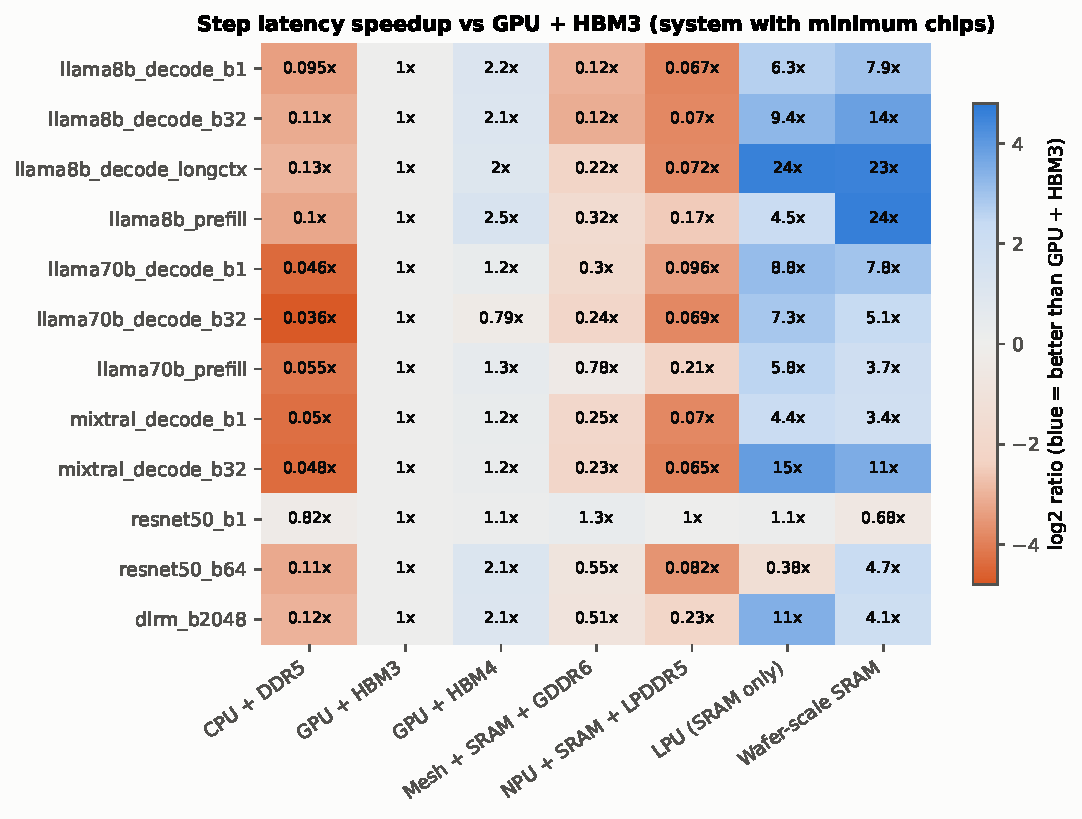
\includegraphics[width=0.55\textwidth]{figures/03_ai_latency_speedup.pdf}
\caption{Step-latency speedup over GPU + HBM3 (two significant figures). Each system uses the minimum number of chips that holds the model state.}
\label{fig:speedup}
\end{figure}



\textbf{Per chip, HBM wins.} Normalized per chip, the LPU-class system delivers about 1/12 of an HBM3 GPU's throughput on Llama-8B and about 1/37 on Llama-70B. On the LLM scenarios only GPU + HBM4 (2.0--2.7\tmx) and the wafer, whose single ``chip'' holds 44\,GiB of SRAM, beat the HBM3 GPU per chip. Batching widens the gap: from batch 1 to 256, GPU throughput per chip grows about 32\tmx, while SRAM systems must add chips to hold the growing KV cache.



\textbf{The bottleneck moves rather than disappears} (Figure~\ref{fig:breakdown}). The LPU-class system spends 68--79\% of its decode time on all-reduce latency and the rest on per-operator synchronization; the wafer is mostly bound by synchronization overhead. Prefill is compute-bound on every DRAM-based system and on a single wafer, except on multi-chip SRAM-only deployments, where all-reduces take 71--92\% of the time. This all-reduce share is an upper bound, since we assume pure tensor parallelism, and its split from per-operator overhead follows the calibrated $h$ and $\tau$.

Small networks expose these fixed costs too. ResNet-50 at batch 1 is overhead-bound on every system except the CPU, so the mesh ($\tau=2\,\mu$s) beats the GPUs ($3\,\mu$s) and the wafer ($5\,\mu$s) is slowest. At batch 64, the single-chip LPU is compute-bound at 188 TFLOPS, while the NPU's 144\,MiB SRAM no longer holds the activations and its traffic spills to LPDDR5. DLRM is compute-bound on the HBM GPUs and gather-bound on GDDR6 and LPDDR5, whose 25\%/45\% row-gather efficiency costs them 2--4\tmx.

\begin{figure}[htbp]
\centering
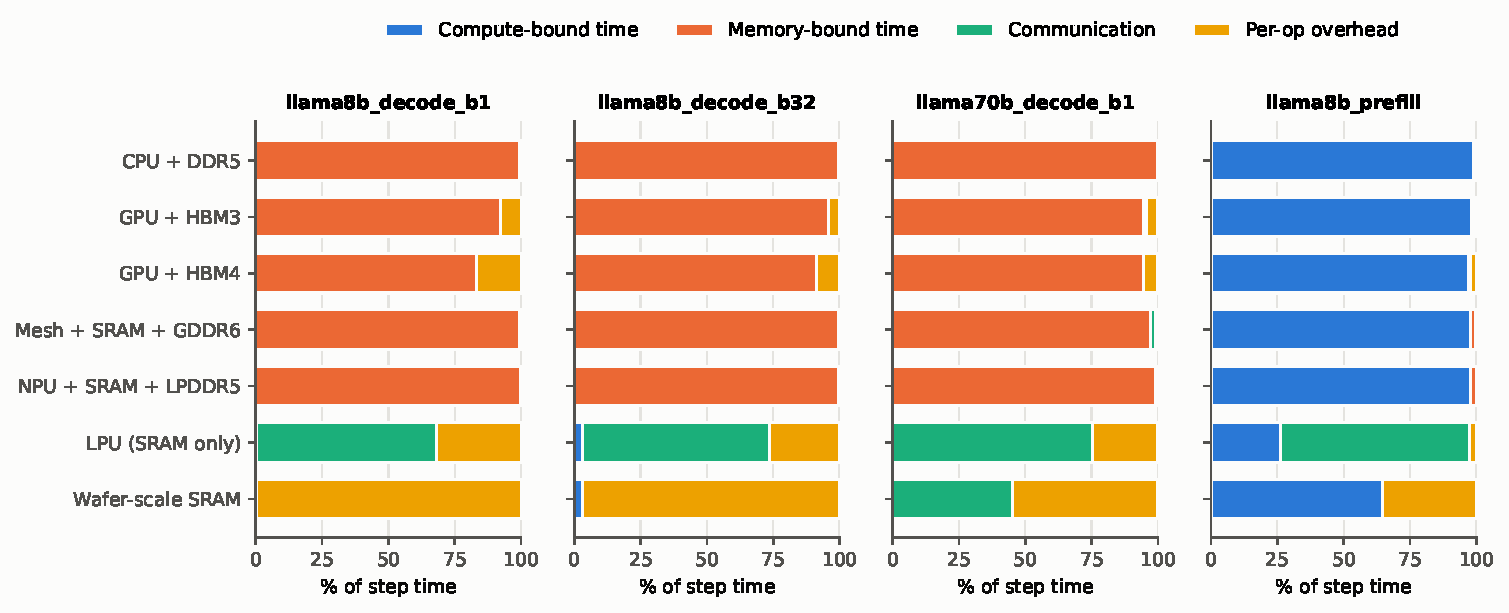
\includegraphics[width=0.78\textwidth]{figures/06_time_breakdown.pdf}
\caption{Where step time goes. DRAM systems are memory-bound in decode and compute-bound in prefill; SRAM-only systems are bound by inter-chip communication and per-operator synchronization.}
\label{fig:breakdown}
\end{figure}

\textbf{Capacity cliffs.} When the KV cache pushes the wafer system from one wafer to two, tensor-parallel communication appears: at batch 128 the step time jumps from 0.69 to 1.62\,ms and throughput per wafer drops 2.3\tmx; at a 32k context it rises from 0.66 to 0.96\,ms and throughput per wafer drops 2.9\tmx. HBM systems degrade smoothly. A 32k context at batch 8 makes the KV cache 34\,GB, larger than the weights, and raises the LPU chip count from 76 to 233.



MoE decouples bandwidth from capacity: at batch 1 Mixtral reads about 26 of its 93\,GB per token, but SRAM-resident designs must still hold all experts (432 LPU-class chips).

\textbf{Energy} (Figure~\ref{fig:energy}). Memory-access energy per token is 13--16\tmx{} lower on SRAM-resident systems than on the HBM3 GPU. Once static power is counted, however, the 76-chip LPU-class system uses 5.2\tmx{} the GPU's energy per Llama-8B token at batch 1 (16\tmx{} on Llama-70B), and the wafer 4.2\tmx{} (8.5\tmx). At batch 32 the HBM GPUs are the most efficient, at 0.17--0.20\,J/token against at least 0.31\,J for every other design.

\begin{figure}[htbp]
\centering
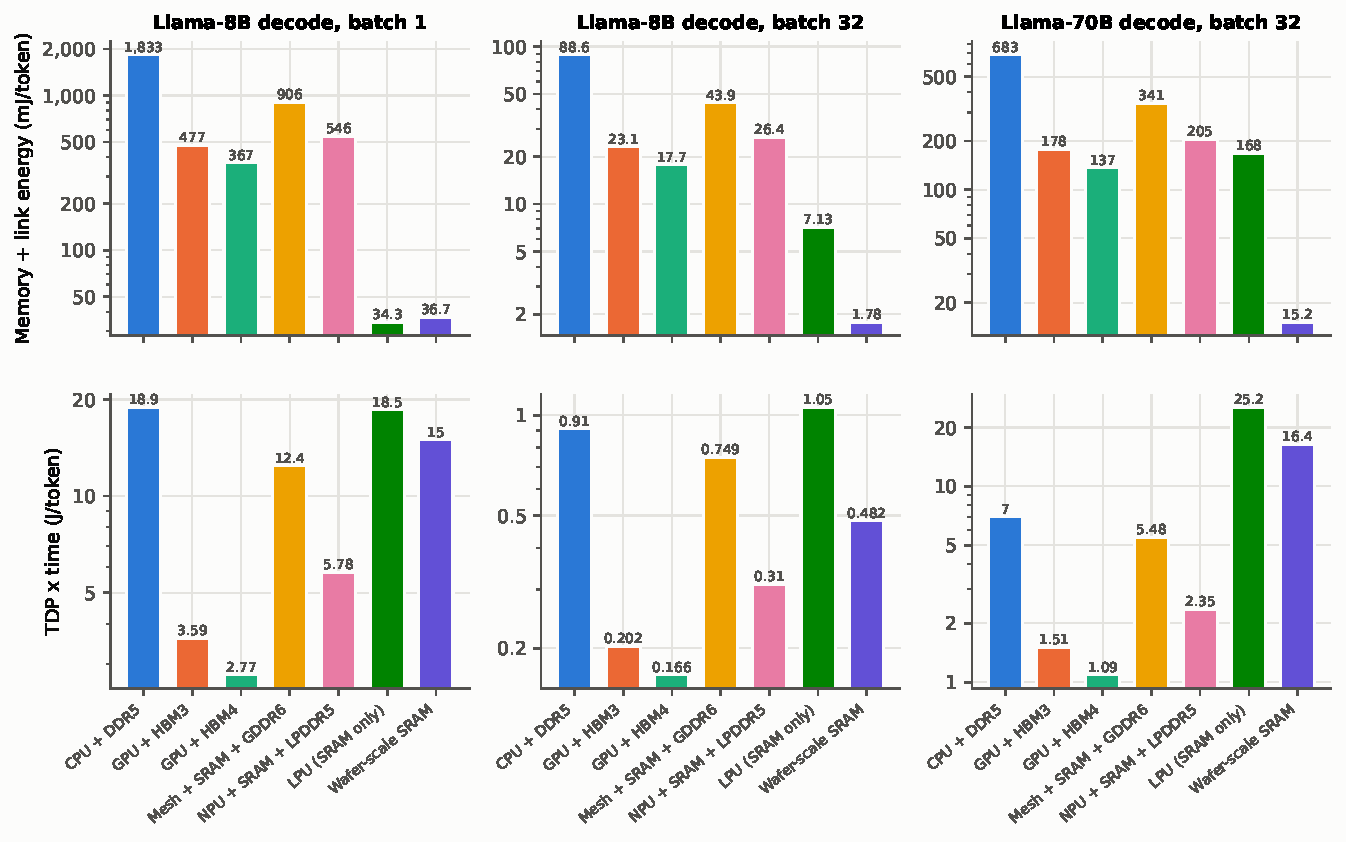
\includegraphics[width=0.78\textwidth]{figures/07_energy.pdf}
\caption{Energy per token. Top: dynamic memory and link energy. Bottom: chips \tmx{} TDP \tmx{} time, an upper bound that includes static power.}
\label{fig:energy}
\end{figure}

%---------------------------------------------------------------------
\subsection{General-Purpose Code (SPEC CPU 2026)}
Seven of the eight benchmarks make only 0.2--2 DRAM accesses per kilo-instruction on 1 core; only lbm (a 542\,MiB lattice sweep, 43 APKI) is bandwidth-heavy. For the other seven, the hot working set fits in every LLC, so DRAM traffic is almost identical across architectures, and IPC follows the LLC hit latency instead (Table~\ref{tab:spec1}).

\begin{table}[htbp]
\centering
\caption{IPC relative to CPU + DDR5, 1 core (APKI on CPU + DDR5), with the 4-core geomeans.}
\label{tab:spec1}
\small
\setlength{\tabcolsep}{4pt}
\begin{tabular}{@{}lrrrrrrrr@{}}
\toprule
Benchmark & APKI & CPU IPC & HBM3 & HBM4 & Mesh & NPU & LPU & Wafer\\
\midrule
stockfish & 0.38 & 3.20 & 0.66 & 0.66 & 0.81 & 0.87 & 0.92 & 0.52\\
sqlite & 0.41 & 3.38 & 0.49 & 0.49 & 0.69 & 0.79 & 0.87 & 0.36\\
omnetpp & 0.20 & 3.22 & 0.28 & 0.28 & 0.47 & 0.61 & 0.71 & 0.18\\
sealcrypto & 0.73 & 3.09 & 0.36 & 0.36 & 0.56 & 0.70 & 0.81 & 0.25\\
nest & 2.04 & 1.86 & 0.23 & 0.23 & 0.41 & 0.56 & 0.71 & 0.15\\
marian & 0.24 & 3.48 & 0.84 & 0.84 & 0.94 & 0.97 & 1.00 & 0.73\\
zstd & 0.54 & 2.80 & 0.47 & 0.47 & 0.66 & 0.77 & 0.88 & 0.33\\
lbm & 43.4 & 1.58 & 0.48 & 0.48 & 0.64 & 0.67 & 0.78 & 0.36\\
\midrule
Geomean & & -- & 0.44 & 0.44 & 0.63 & 0.73 & 0.83 & 0.32\\
Geomean, 4 cores & & -- & 0.53 & 0.52 & 0.71 & 0.70 & 0.83 & 0.39\\
LLC hit (cycles) & & 56 & 480 & 480 & 240 & 160 & 120 & 800\\
\bottomrule
\end{tabular}
\end{table}





\textbf{Latency, not bandwidth, decides general-purpose code.} SPEC-style code issues dependent, irregular accesses with little memory-level parallelism. A large SRAM that is 120--200\,ns away costs pointer-chasing codes the most: omnetpp and nest run at 0.28\tmx{} and 0.23\tmx{} on the GPUs and 0.18\tmx{} and 0.15\tmx{} on the wafer, even though the SRAM never misses. Compute-dense codes with small hot sets (marian, stockfish) lose least.

\textbf{HBM bandwidth buys nothing here.} GPU + HBM4 has 2.5\tmx{} the DRAM bandwidth and 2.5\tmx{} the LLC of GPU + HBM3, yet its IPC is within 1\% on every benchmark except 4-core lbm, where it is 10\% slower. The cores cannot generate enough parallel misses: at most $4\times32$ 64\,B misses (8\,KiB) are in flight, so even 4-core lbm uses only 61--67\,GB/s of HBM. Loaded DRAM read latency is similar on HBM (35--50\,ns) and DDR5 (28--73\,ns), so the GPUs' IPC deficit comes from the 120\,ns LLC hit latency, not from DRAM. Throughput-oriented GPUs hide such latencies with many threads, which this study does not model.



\textbf{Capacity helps only the bandwidth-heavy benchmark.} lbm's 101 APKI on 4 cores falls to 32--36 with the 208--232\,MiB LLCs of the mesh and LPU, which recover 0.81--0.87\tmx{} of CPU IPC, and to 29 with the wafer's 1\,GiB LLC. The NPU's 144\,MiB does not hold the working set, so the full stream goes to LPDDR5, its loaded read latency reaches 126\,ns (60\,ns on DDR5), and IPC falls to 0.45\tmx.

\textbf{The ranking follows SRAM latency, not AI performance.} Of the two fastest AI systems, the LPU (30\,ns SRAM) is the least affected non-CPU design (0.83\tmx) and the wafer (200\,ns) the most affected (0.32\tmx).

%---------------------------------------------------------------------
\subsection{Memory Access-Pattern Characterization}
\textbf{Trace level.} The L2-miss traces (Figure~\ref{fig:spatial}, Table~\ref{tab:pattern}) fall into four families:
\begin{itemize}
\item \emph{Streams:} marian reads its weights as one sequential stream (99\% stream share, no re-references, the most regular gaps); sealcrypto is 100\% streams, interleaved more than 1\,MiB apart, in short bursts (the burstiest gaps, CV 30).
\item \emph{Interleaved streams:} lbm sweeps its lattice with several streams; consecutive misses alternate between them, so no miss is to the next line, yet 70\% stay in the same 4\,KiB page. At 58 MPKI it is the only bandwidth-bound trace.
\item \emph{Scattered reuse:} omnetpp (89\% of misses re-referenced) and nest (73\%), the pointer-chasing codes that lose most IPC on slow LLCs.
\item \emph{Sweep plus scatter:} stockfish, sqlite and zstd.
\end{itemize}
Re-referenced misses hit in every LLC, which is why DRAM traffic barely changes across architectures.

\begin{figure}[htbp]
\centering
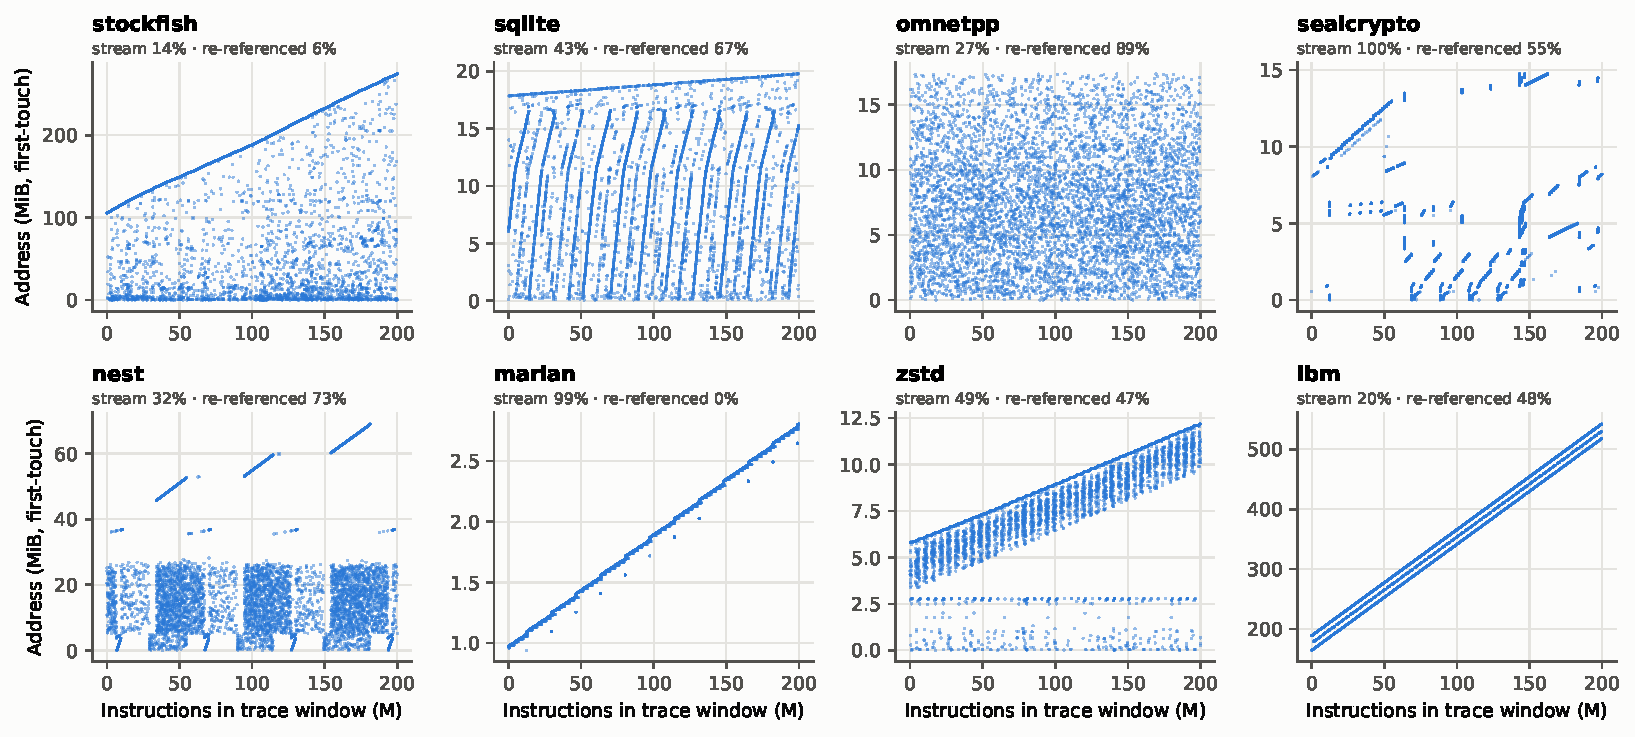
\includegraphics[width=0.78\textwidth]{figures/12_access_spatial.pdf}
\caption{Address of every L2 miss over the 200M-instruction trace window (6,000 evenly spaced samples; first-touch physical addresses).}
\label{fig:spatial}
\end{figure}

\begin{table}[htbp]
\centering
\caption{Trace-level access-pattern metrics (L2 misses).}
\label{tab:pattern}
\small
\begin{tabular}{@{}lrrrrrrr@{}}
\toprule
Benchmark & MPKI & Mean / median gap & CV & Next & Page & Stream & Re-ref\\
\midrule
stockfish & 0.39 & 2,556 / 2,132 & 1.1 & 12\% & 3\% & 14\% & 6\%\\
sqlite & 2.34 & 428 / 39 & 3.5 & 30\% & 35\% & 43\% & 67\%\\
omnetpp & 5.47 & 183 / 32 & 2.3 & 17\% & 38\% & 27\% & 89\%\\
sealcrypto & 2.63 & 381 / 46 & 29.9 & 80\% & 0\% & 100\% & 55\%\\
nest & 11.47 & 87 / 37 & 1.9 & 19\% & 35\% & 32\% & 73\%\\
marian & 0.15 & 6,667 / 9,168 & 0.6 & 85\% & 0\% & 99\% & 0\%\\
zstd & 1.19 & 841 / 443 & 3.2 & 25\% & 1\% & 49\% & 47\%\\
lbm & 57.89 & 17 / 1 & 5.9 & 0\% & 70\% & 20\% & 48\%\\
\bottomrule
\end{tabular}\\[2pt]
{\footnotesize Gap in instructions between misses. Next = next 64\,B line; Page = other line in the same 4\,KiB page; Stream = stream share; Re-ref = re-reference share.}
\end{table}

\textbf{At the memory controllers.} Each benchmark keeps a recognisable inter-request timing signature on every system; on the GPU the gaps grow, because each miss first pays the 120\,ns LLC hit latency. Table~\ref{tab:mc} gives the average controller throughput and the PSD class, and Figure~\ref{fig:psd} the spectra.



\begin{table}[htbp]
\centering
\caption{Memory-controller throughput (GB/s) and PSD slope $\beta$ with class (S = stationary, M = monofractal, MF = multifractal, AP = anti-persistent). Classes also depend on the half-range slopes $\beta_{\mathrm{lo}}$ and $\beta_{\mathrm{hi}}$ (not shown), so equal $\beta$ can give different classes.}
\label{tab:mc}
\scriptsize
\setlength{\tabcolsep}{3pt}
\begin{tabular}{@{}lrrrrrcrrrrr@{}}
\toprule
 & \multicolumn{5}{c}{Throughput (GB/s)} & & \multicolumn{5}{c}{$\beta$ (class)}\\
\cmidrule{2-6}\cmidrule{8-12}
Benchmark & DDR5 & HBM3 & HBM4 & GDDR6 & LPDDR5 & & DDR5 & HBM3 & HBM4 & GDDR6 & LPDDR5\\
\midrule
stockfish & 0.44 & 0.31 & 0.31 & 0.37 & 0.39 & & 0.27 M & 0.27 S & 0.27 S & 0.30 M & 0.31 M\\
sqlite & 0.61 & 0.32 & 0.32 & 0.43 & 0.49 & & 0.31 MF & 0.34 M & 0.34 M & 0.32 M & 0.33 M\\
omnetpp & 0.45 & 0.12 & 0.12 & 0.21 & 0.27 & & 0.18 S & 0.18 S & 0.18 S & 0.18 S & 0.20 M\\
sealcrypto & 0.86 & 0.35 & 0.35 & 0.51 & 0.60 & & 0.09 S & 0.05 S & 0.05 S & 0.09 S & 0.10 S\\
nest & 1.95 & 0.61 & 0.60 & 0.98 & 1.17 & & 0.37 MF & 0.12 MF & 0.10 MF & 0.17 MF & 0.42 MF\\
marian & 0.13 & 0.11 & 0.11 & 0.12 & 0.12 & & 1.04 MF & 1.08 MF & 0.98 MF & 0.97 MF & 1.37 MF\\
zstd & 0.45 & 0.21 & 0.21 & 0.30 & 0.34 & & 0.53 M & 0.54 MF & 0.54 MF & 0.54 M & 0.55 M\\
lbm & 15.95 & 8.42 & 5.96 & 8.21 & 8.26 & & $-$0.43 AP & $-$0.20 S & $-$0.19 S & $-$0.28 S & $-$0.09 S\\
\bottomrule
\end{tabular}
\end{table}

\begin{figure}[htbp]
\centering
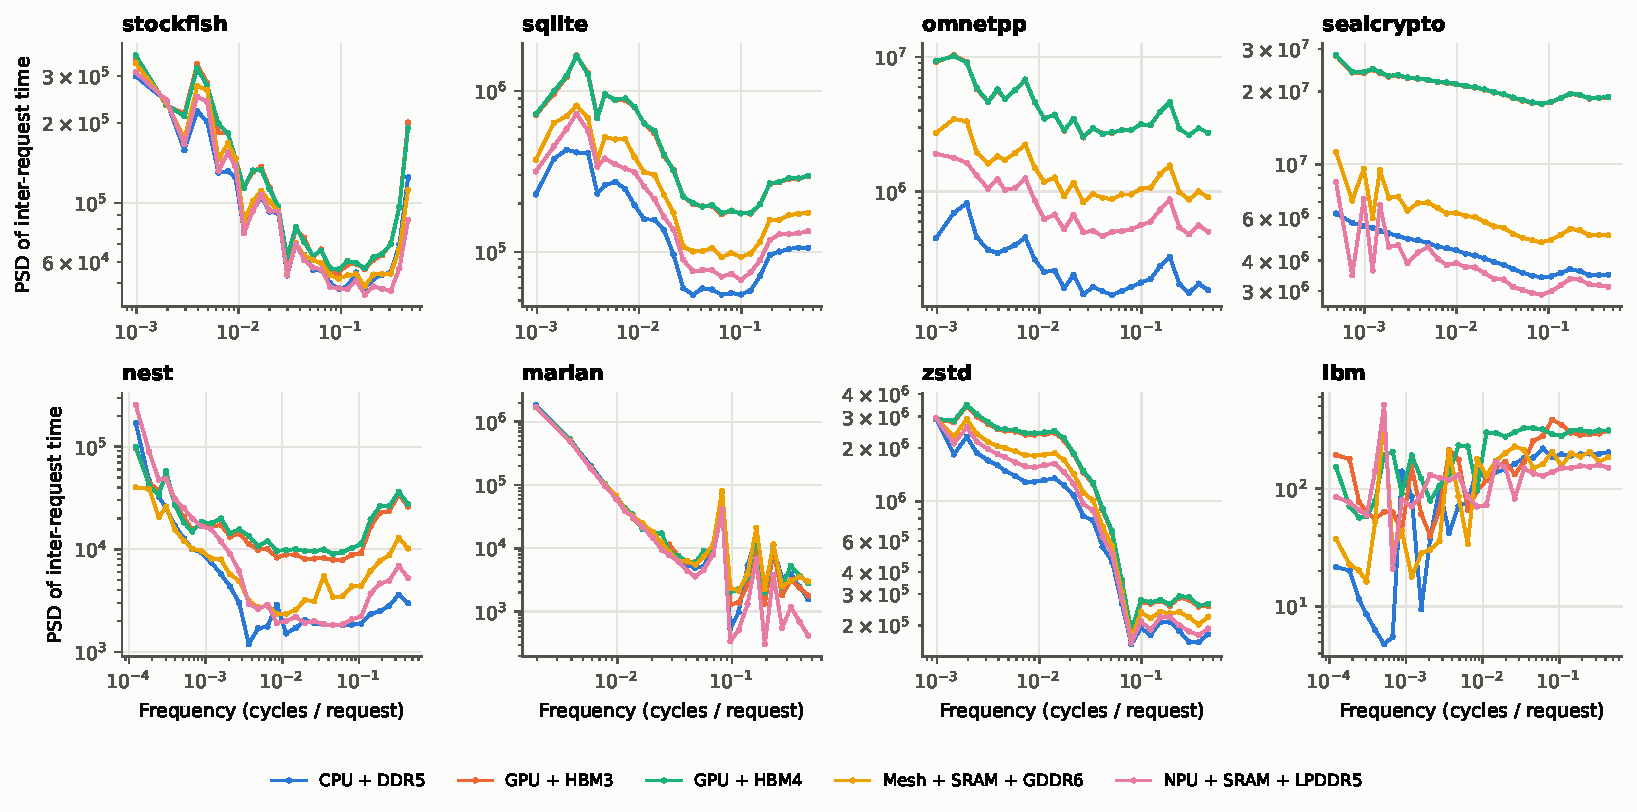
\includegraphics[width=0.78\textwidth]{figures/14_mc_psd.pdf}
\caption{Log-log PSD of the inter-request time at the memory controllers per benchmark and DRAM-backed architecture (cf.~\cite{agarwal2025}); frequency in cycles per request, i.e.\ per sample of the series (Nyquist 0.5). marian's $\approx$4,250 requests limit its lowest resolvable frequency.}
\label{fig:psd}
\end{figure}

\textbf{The program, not the memory system, sets the shape of the request stream.} For five of the eight benchmarks, $\beta$ varies by at most 0.05 across the five memory systems, and 33 of the 40 benchmark--system pairs share their benchmark's majority class. This holds because seven of the eight hot sets fit in every LLC, so mostly compulsory misses reach DRAM. Unlike in the NoC study~\cite{agarwal2025}, where cache and buffer sizes changed the class, the memory system here mainly rescales the timing. sealcrypto is stationary everywhere and omnetpp on four of the five systems; stockfish, sqlite and zstd are mostly monofractal; marian and nest are multifractal, and marian shows a $1/f^2$ low-frequency trend and a period of about 13 requests. lbm, whose working set does not fit, changes class (anti-persistent on DDR5, stationary elsewhere). The class changes of stockfish and zstd between narrow DRAMs and HBM may partly come from merging many more channels into one series.

\textbf{Throughput follows the core, not the DRAM.} Controller throughput is highest on CPU + DDR5 for every benchmark (0.13--16\,GB/s) and 1.2--3.8\tmx{} lower on the GPUs. Even lbm draws only 6--8\,GB/s from HBM systems with terabytes per second of peak bandwidth. Because the analysis window is the second half of the run \emph{time}, it covers different instructions on each system: throughputs are rates, and differences at equal IPC reflect the sampled program phase and, for lbm on HBM3 and HBM4, likely also LLC capacity (in a separate 20M-instruction replay, the 50\,MiB LLC wrote back 85,138 dirty lines that the 128\,MiB one kept).

\textbf{Row-buffer locality needs both a spatial pattern and few channels} (Figure~\ref{fig:locality}). Only sealcrypto, lbm, nest and, on the 2-channel host memory, zstd reach high row-hit rates. For sealcrypto and lbm the hit rate is 2--17\% on HBM4 (128 channels), 7--30\% on HBM3 (64), 20--49\% on GDDR6 (8), 22--55\% on DDR5 (16), 27--73\% on LPDDR5 (8) and 38--82\% on the 2-channel host DDR5. 64\,B interleaving spreads each stream across all channels, so a 4\,KiB page touches each HBM channel at most once: wide AI memory systems turn even sequential streams into row misses. marian's near-zero hit rate despite its pure stream, and the different hit rates of the LPU and wafer on the same host DDR5, remain unexplained by this study.

\begin{figure}[htbp]
\centering
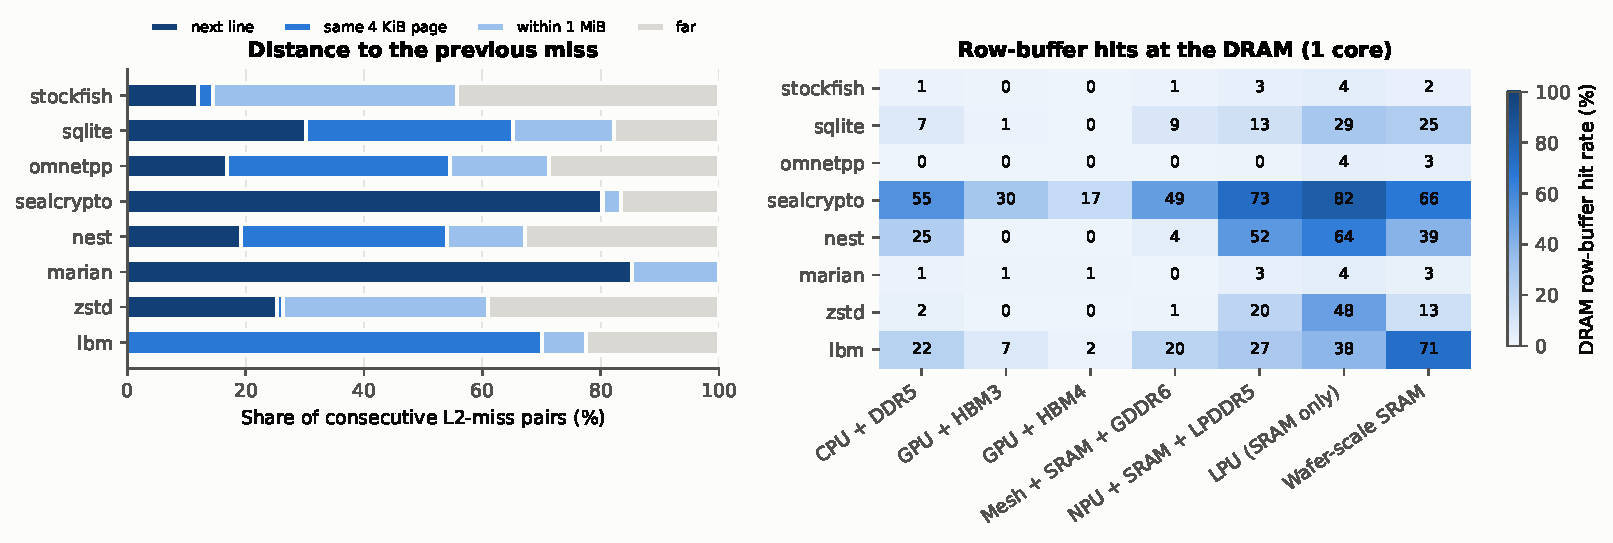
\includegraphics[width=0.78\textwidth]{figures/15_locality.pdf}
\caption{Left: distance of each L2 miss to the previous one (trace level). Right: DRAM row-buffer hit rate in the 1-core replays (100M instructions); the SRAM-only designs reach only a 2-channel host DDR5.}
\label{fig:locality}
\end{figure}

%---------------------------------------------------------------------
\subsection{Limitations}
Architecture parameters are public-specification class values, and the SRAM-only systems' overhead and hop latency are tuned to published token rates, so absolute numbers are indicative. The AI model is analytical on top of cycle-accurate DRAM, with pure tensor parallelism (an upper bound on communication), no GPU shared-memory staging and 16-bit weights; compute, links and overheads differ between chip classes. Each SPEC benchmark contributes one 200M-instruction window in LLVM IR instructions; the 4-core runs use a short warm-up with lockstep copies, the core has no prefetcher, and the IPC ratios scale with the assumed SRAM latencies (30--200\,ns). The controller-level PSD merges all channels into one series and analyses the second half of the run time rather than a fixed instruction range.
\newpage

%=====================================================================
\section{Conclusion}\label{sec:conclusion}
%=====================================================================
This project built a reproducible framework that evaluates the memory systems of seven AI-chip archetypes on AI inference and on general-purpose code, with one cycle-accurate DRAM substrate (Ramulator~2.1), an LLVM-based tracer for SPEC CPU~2026, and a controller-level access-pattern analysis. The main conclusions are:
\begin{enumerate}
\item \textbf{Decode is memory-bound, prefill compute-bound}: 83--100\% of batch-1 decode time on DRAM-based designs is memory time, and speed tracks \emph{achieved}, not pin, bandwidth.
\item \textbf{Access pattern matters as much as peak bandwidth}: on random 64\,B accesses HBM keeps only 46--58\%, LPDDR5 45\% and GDDR6 24\% of its bandwidth (DDR5 86\%).
\item \textbf{SRAM-only designs buy latency with chips}: 6.3--8.8\tmx{} faster batch-1 Llama decode, but the LPU-class design needs 76--654 chips, delivers 1/12--1/37 of an HBM3 GPU's throughput per chip and uses 5--16\tmx{} its energy per token.
\item \textbf{On general-purpose code, IPC follows LLC latency}: 0.32--0.83\tmx{} the geometric-mean IPC of a CPU with DDR5, with HBM4 no better than HBM3.
\item \textbf{The program sets the shape of the request stream} when its hot set fits every LLC, and wide memory systems turn even sequential streams into row misses.
\end{enumerate}
Overall, HBM-based GPUs remain the most balanced choice: good latency, the best throughput per watt on LLM decode and graceful scaling with context and batch. SRAM-only systems are a latency play for interactive single-stream decode of models that fit their aggregate SRAM.

\textbf{Future work.} Natural extensions are quantized (8- and 4-bit) weights, which help capacity-limited SRAM designs most; hybrid pipeline and tensor parallelism; a prefetching, multithreaded core for the SPEC study; per-channel spectra with instruction-aligned windows; and using the PSD class to guide memory-controller scheduling.
\newpage

%%%***************************************************************************************
\settocbibname{References}
\bibliography{Myreferences}

\end{document}
